% LINGI2255 - Software Development Project
% Final report
\documentclass[11pt, a4paper]{article}   	% use "amsart" instead of "article" for AMSLaTeX format
\usepackage[T1]{fontenc}
\usepackage[utf8]{inputenc}
\usepackage{lmodern}
\usepackage[UKenglish]{babel}
\usepackage{graphicx}

\usepackage{amssymb}
\usepackage{xcolor}
\usepackage{hyperref}
\usepackage{url}
\usepackage{csquotes}
\usepackage{enumitem}
\usepackage{lipsum}
\usepackage{listings}
\usepackage{textcomp}
\lstset{language=Python}

\newcommand{\tbf}[1]{\textbf{#1}}
\newcommand{\tit}[1]{\textit{#1}}
\newcommand{\noi}{\noindent}
\newcommand{\shellcmd}[1]{\\\indent\indent\texttt{\footnotesize\$ #1}\\}
\newcommand{\vshellcmd}[1]{\\\indent\indent\texttt{\footnotesize(venv)\$ #1}\\}
\newcommand{\pcmd}[1]{\\\indent\indent\texttt{\footnotesize> > > #1}\\}

\lstset{%
    inputencoding=utf8,
        extendedchars=true,
        literate=%
        {é}{{\'{e}}}1
        {è}{{\`{e}}}1
        {ê}{{\^{e}}}1
        {ë}{{\¨{e}}}1
        {û}{{\^{u}}}1
        {ù}{{\`{u}}}1
        {â}{{\^{a}}}1
        {à}{{\`{a}}}1
        {î}{{\^{i}}}1
        {ô}{{\^{o}}}1
        {ç}{{\c{c}}}1
        {Ç}{{\c{C}}}1
        {É}{{\'{E}}}1
        {Ê}{{\^{E}}}1
        {À}{{\`{A}}}1
        {Â}{{\^{A}}}1
        {Î}{{\^{I}}}1
}

\title{Brief Article}
\author{The Author}
%\date{}							% Activate to display a given date or no date

\begin{document}
%\maketitle

%%%%%% Section
\section{Introduction}

%%%%%% Section
\section{Product}

%\subsection{Features}

\input{statistics.texpart}

%%%%%% Section
\section{Changes from previous reports}

%%%%%% Section
\section{Technical discussion}

\subsection{Virtual Environment}

We use \texttt{pyvenv}, a tool that can create virtual environment in \texttt{Python}, to keep the dependencies required by our project in a single place. It creates a folder which contains all the necessary executables to use the packages that our project will need. To create the virtual environment :
\shellcmd{pyvenv venv}
To activate the environment :
\shellcmd{source venv/bin/activate}
Once your virtual environment installed and activated, you can install the dependencies of \texttt{Care4Care}. All the dependencies are listed in the file requirements.txt. You can install all of them with the following command:
\vshellcmd{pip install -r requirements.txt}

\subsection{Create the database}
Once you're in a proper virtual environment with all dependencies installed, you can create the database. To do so, you can go in the root of our \texttt{Django} project and use the built-in command :
\vshellcmd{./manager.py syncdb}
At the end, you will ask to create a ``super user'', you can create a user ``care4care''. If you want to populate the database with some demo datas, you can run :
\vshellcmd{./manager.py loaddata data\_demo.json}

\subsection{Run the project}
One you're in the virtual environment with all dependencies installed and the dabatase created, you can launch the development server :
\vshellcmd{./manager.py runserver}
When the server is launched, you can browse the website in your browser at \url{http://localhost:8000}.

\subsection{File hierarchy}
The project is divised in three ``Django applications'' wich are differents folders in our project :
\begin{description}[noitemsep]
\item[- main] contains everything about users management
\item[- branch] contains everything about branch and jobs (demands and offers)
\item[- news] contains everything about the news system
\end{description}

Each of these ``Django applications'' contains typic files/folders :
\begin{description}[noitemsep]
\item[- migrations/] is a folder containing migrations files. This is the Django’s way of propagating changes we make in our models (adding a field, deleting a model, etc.) into our database schema.
\item[- templates/] is a folder containing our templates. A template is simply a text file (ofter HTML). It contains variables, which get replaced with values when the template is evaluated, and tags, which control the logic of the template.
\item[- Templatestags/] is a folder in wich we will extend the template engine by defining custom tags, and then make them available in our templates.
\item[- static/] is a folder in wich we will put every static files (images, javascript, photos, etc.) used by the application.
\item[- \_\_init\_\_.py] used to mark the folder on disk as Python package directory.
\item[- admin.py] contains all the logic for the auto-generated django-admin.
\item[- forms.py] contains all the forms used by the ``Django application'' and the validation logic.
\item[- models.py] contains all the models used by the ``Django application''. Models are the source of information about data. Each attribute of a model represents a database field. 
\item[- tests.py] contains unit tests.
\item[- urls.py] contains every URLs available for the ``Django application''.
\item[- views.py] contains the logic of every views (linked to an URL) for the ``Django application''.
\end{description}

There is some more specific folders in the root of our project that need to be describe :
\begin{description}[noitemsep]
\item[- care4care/] contains the settings.py file where you can define all settings relative to our project.
\item[- templates/] contains templates that are linked to a third-party application.
\item[- static/] contains all static files not related to a specific application but more about the whole project.
\item[- media\_root/] contains every files uploaded by users via the website.
\item[- locale/] contains translations (i18n) of the project.
\end{description}

And there is some more specific files in the root of our project that need to be describe :
\begin{description}[noitemsep]

\item[- make\_locale.sh] generates translations .po files into ``locale/''. These files contains every sentences to be translated.
\item[- compile\_locale.sh] compiles translations .po files into usable translations .mo files.
\item[- manage.py] is generated by Django. This is the command-line utility for administrative tasks. 
\item[- start.sh] will run the project in a gunicorn server for production environment.
\end{description}

\subsection{Django : How does it works ? A simple example}

To understand how Django works, we'll use as an example the page that allows an user to add an emergency contact. Everything shown here is present in our code in the application ``main''.

\subsubsection{Models}
First, we have to create a model (wich is represented by a Class) in \texttt{models.py}:

\begin{lstlisting}[language=Python, basicstyle=\footnotesize]
PRIORITY = (
    (1, _("A contacter en premier")), # To contact first
    (2, _("A contacter")), # To contact 
    (3, _("A contacter en dernier")) # To contact ultimately
    )

class EmergencyContact(CommonInfo):
    user = models.ForeignKey('User', related_name="emergency_contacts")
    order = models.IntegerField(default=0, \
      verbose_name=_("Ordre de priorité"), choices=PRIORITY)

    class Meta:
        ordering = ['order']
\end{lstlisting}

Class EmergencyContact inherits from class CommonInfo. CommonInfo contains fields : first\_name, last\_name, location, latitude, longitude, phone\_number, mobile\_number and languages. So EmergencyContact already got all these attributes. Plus, we add two other : user and order. User is a ForeignKey to the class User. It will be useful to know wich User is associated with an emergency contact. And the order field is useful to know wich emergency contact you should contact first.


This class will create all necessary entries in the databases. It also gives us an easy API to make request to the database. So, if we want to get all the EmergencyContact of user id number 4, we can write:
\pcmd{EmergencyContact.objects.filter(user\_\_id=4).all()}

In the Meta class, we wrote ``ordering = ['order']'', this has the effect of sorting the results of our requests per the field ``order''.

\subsubsection{View}
The view is the logic of the page.

\begin{lstlisting}[language=Python, basicstyle=\footnotesize]
# in forms.py
class EmergencyContactCreateForm(forms.ModelForm):
    class Meta:
        model = EmergencyContact
        exclude = ['user', 'latitude', 'longitude']

# in views.py
class AddEmergencyContact(CreateView):
    """A view for add an emergency_contact"""
    template_name = 'profile/emergency_contact.html'
    form_class = EmergencyContactCreateForm
    model = EmergencyContact

    @method_decorator(login_required)
    def dispatch(self, *args, **kwargs):
        obj = self.get_object()
        if obj.id != self.request.user.id and not self.request.user.is_superuser:
            return redirect(obj.get_absolute_url())
        return super(AddEmergencyContact, self).dispatch(*args, **kwargs)

    def get_object(self, queryset=None):
        return User.objects.get(pk=self.kwargs['user_id'])

    def form_valid(self, form):
        form.instance.user = User.objects.get(pk=self.kwargs['user_id'])
        return super(AddEmergencyContact, self).form_valid(form)

    def get_success_url(self):
        return self.get_object().get_absolute_url()
\end{lstlisting}

We will use a Generic View (CreateView) to create a new Emergency Contact. Since the administrator (superuser) can be able to add an emergency contact to any user, we will have to specify for wich user we create an emergency contact. To do so, we will give the user id in the url linked to this view (see next section). We can get the number id via ``self.kwargs['user\_id']''. Since this will be useful, we define a method \texttt{get\_object} that will get the user object in database. Then, we will override the dispatch method. In this method, we will first add the method decorator \texttt{login\_required}. This decorator will assure that the user is connected. If not, it will brings the user to the login page. In the method, we will check that the user have got enough right to create an emergency contact for the user (self.get\_object). 

We specify the form via the field form\_class. So we created a class EmergencyContactCreateForm. This form is an ModelForm, so it will be automatically generated from the model EmergencyContact as we can read in his Meta class. We can see that we exclude three fields that we don't want here : user, latitude and longitude. So we will ask the user all fields of the model class EmergencyContact except these three.

We override the method form\_valid to link the current user (self.get\_object) with the emergency contact in creation.

At least, we override the method \texttt{get\_success\_url}. When the form is valid, the user will be redirect the profile of the user. If the form is not valid, the CreateView logic will point out the error to the user and ask him to correct it.

\subsubsection{URLs}

In the file \texttt{urls\_profile.py} (extension of \texttt{urls.py}), we will add the following entry in the urlpatterns :

\begin{lstlisting}[language=Python, basicstyle=\footnotesize]
  url(r'^profile/add_emergency_contact/(?P<user_id>\d+)/',
      AddEmergencyContact.as_view(),
      name='add_emergency_contact'), 
\end{lstlisting}

We can find the famous ``user\_id'' that will be use in the method \texttt{get\_object} in our view. Also, we give a name to our url. This is usefull to not remember the used url since we will be able to write the url in a template with the templatetag url : ``\{\% url 'add\_emergency\_contact' request.user.id \%\}''.

\subsubsection{Template}

The final step is to write the template specified in our view : \texttt{'profile/emergency\_contact.html'}:

\begin{lstlisting}[language=HTML, basicstyle=\footnotesize]





[..]
    <form action="." role="form" method="post">
      
       [..]
          
        [..]
        <button type="submit" class="btn btn-success btn-lg btn-block">
             &nbsp; </button>
        [..]
    </form>
[..]

\end{lstlisting}

We can see that render our form is easy as ``\{\% bootstrap\_form form \%\}''. We just need the <form> and a submit button. The rest is for the style of the page.

And that's all, we have created a page with the possibility of creating an emergency contact linked to a user :

\begin{figure}[!ht]
   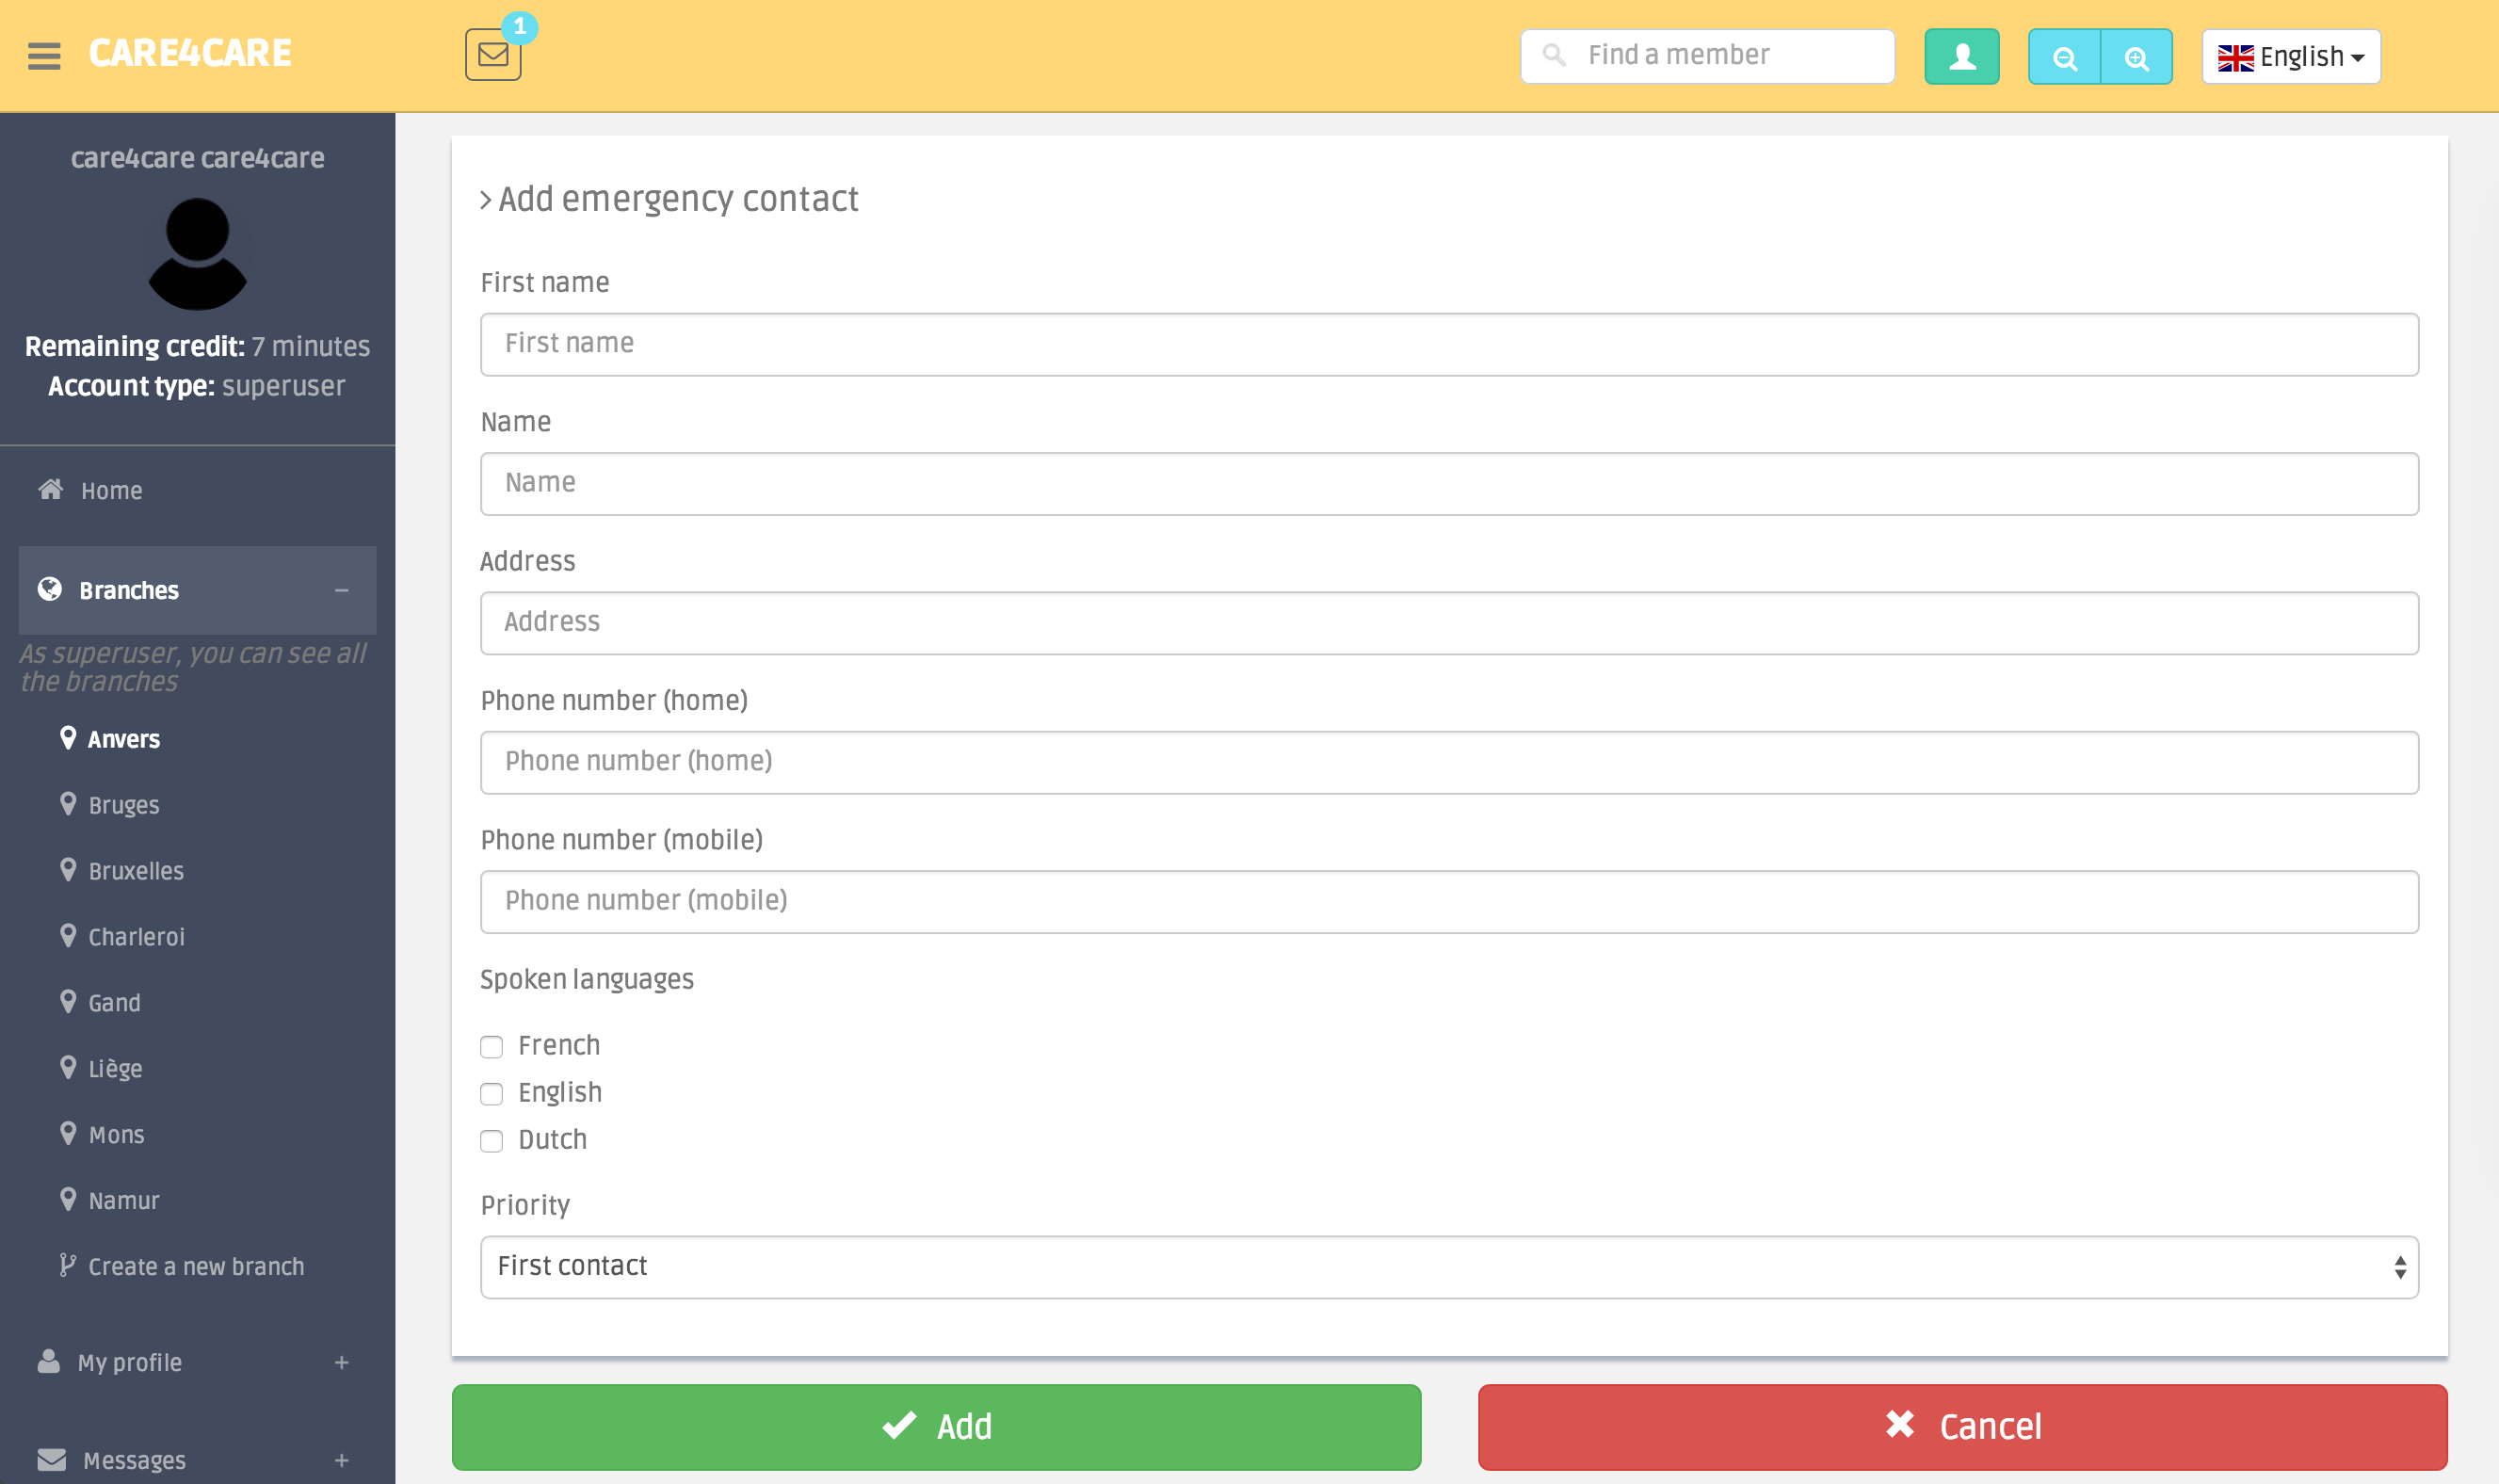
\includegraphics[height=220px]{addec.png}
\end{figure}


%%%%%% Section
\section{Conclusion}

\end{document}
